\begin{enumerate}
\subsection*{I. Conjugaison dans $G$}
\item Soit $f\in G$.
\[
 \forall t\in \R,\;  f'(t) > 0 \; \text{ et } \; f(t+2\pi) = f(t) + 2\pi.
\]

\begin{enumerate}
  \item Considérons une propriété $\mathcal{P}_n$ attachée à un entier quelconque $n\in \Z$:
\[
  \mathcal{P}_n: \hspace{1cm} \forall x \in \R, \; f(x + 2n \pi) = f(x) + 2n \pi.
\]
La propriété $\mathcal{P}_0$ est évidente. Pour tout $n \in \Z$, l'implication $\mathcal{P}_n \Rightarrow \mathcal{P}_{n+1}$ vient de la relation de pseudo-périodicité appliquée en $t = x + 2n\pi$. De même, $\mathcal{P}_n \Rightarrow \mathcal{P}_{n-1}$ vient de la relation appliquée en $t = x + 2(n-1)\pi$:
\begin{multline*}
  f(x+2n\pi) = f(x+2(n-1)\pi + 2\pi) = f(x+2(n-1)\pi) + 2\pi \\
  \Rightarrow f(x+2(n-1)\pi) = f(x+2n\pi) - 2\pi = f(x) + 2n\pi -2\pi = f(x) +2(n-1)\pi.
\end{multline*}
On en déduit par  récurrence que $\mathcal{P}_n$ est vraie pour tous les $n\in \Z$.

  \item Pour un réel $t$ quelconque, considérons la partie entière $n = \lfloor \frac{t}{2\pi} \rfloor$.
\[
  n \leq \frac{t}{2\pi} < n+1 
  \Rightarrow 2n\pi \leq t < 2n\pi + 2\pi
  \Rightarrow 0 \leq t - 2n\pi < 2\pi .
\]
On utilise ensuite la stricte croissante de $f$ (car $f'$ à valeurs $>0$) et le résultat de la première question:
\begin{multline*}
  f(0) \leq f(t) - 2n\pi < f(2\pi)
  \Rightarrow f(0) + \underset{>t - 2\pi}{\underbrace{2n\pi}} \leq f(t) < f(2\pi) + \underset{\leq t}{\underbrace{2n\pi}} \\
  \Rightarrow f(0) + t - 2\pi < f(t) < f(2\pi) + t.
\end{multline*}

  \item On doit montrer que $f\in G$ est bijective. Comme $f'$ est à valeurs strictement positives, $f$ est strictement croissante donc injective. Pour montrer la surjectivité, considérons un réel $y$ quelconque. D'après b.
\[
  \begin{aligned}
    \left( \forall t \in \R, \; f(t) \leq f(2\pi) + t \right) &\Rightarrow \exists a \in \R \text{ tq } f(a) \leq  y \\
    \left( \forall t \in \R, \; f(0) + t -2\pi \leq f(t) \right) &\Rightarrow \exists b \in \R \text{ tq } y \leq f(b)
  \end{aligned} .
\]
La fonction $f$ étant continue, le théorème des valeurs intermédiaires justifie l'existence d'un réel $x$ entre $a$ et $b$ tel que $f(x) = y$.
\end{enumerate}

\item Soit $f$ et $g$ dans $G$. D'après le théorème de la dérivée de la bijection réciproque:
\[
  {f^{-1}}' = \frac{1}{f'\circ f^{-1}}
\]
est à valeurs strictement positives et continue donc $f^{-1} \in \Cont^1(\R,\R)$.\newline
Pour tout réel $x$, appliquons la relation de pseudo-périodicité de $f$ en $f^{-1}(x)$:
\[
  f(f^{-1}(x) + 2\pi) = f(f^{-1}(x)) + 2\pi = x +2\pi \Rightarrow f^{-1}(x) + 2\pi = f^{-1}(x +2\pi)
\]
en composant par $f^{-1}$. On en déduit $f^{-1} \in G$.\newline
Montrons que $f \circ g \in G$. Pour tout réel $t$:
\[
\left.
  \begin{aligned}
&(f\circ g)'(t) = g'(t)\, f'(g(t)) > 0\\ 
&f\circ g( t + 2\pi) = f(g(t) + 2\pi) = f(g(t)) + 2\pi.
  \end{aligned}
  \right\rbrace
  \Rightarrow f \circ g \in G .
\]
Cette question montre que $(G,\circ)$ est un groupe.

\item Soit $h\in \Cont^{1}(\R, \R_{+}^{*})$ une fonction $2\pi$-périodique à valeurs strictement positives.
\begin{enumerate}
  \item Si $h$ admet une primitive dans $G$, c'est à dire s'il existe $\varphi \in G$ tel que $\varphi' = h$. Alors
\[
  \int_0^{2\pi}h(t)\,dt = \left[ \varphi \right]_0^{2\pi} = \varphi(2\pi) - \varphi(0) = 2\pi
\]
par définition des éléments de $G$.\newline
Réciproquement, supposons $\int_0^{2\pi}h(t)\,dt = 2\pi$ et considérons une primitive $\varphi$ de $h$. Alors $\varphi$ est $\Cont ^2$ car $h$ est $\Cont^1$. De plus $\varphi'$ est à valeurs strictement positives comme $h$. Pour la pseudo-périodicité, considérons $T(t) = \varphi(t+2\pi) - \varphi(t)$.
\[
\forall t \in \R, \; T'(t) = h(2+2\pi) - h(t) = 0 \text{ (périodicité de $h$)}.
\]
Donc la fonction $T$ est constante d'où
\[
\forall t \in \R,\;  \varphi(t+2\pi) - \varphi(t) = T(0) = \varphi(2\pi) - \varphi(t) = \int_0^{2\pi}h(t)\,dt = 2\pi. 
\]

  \item Comme $h$ est continue à valeurs strictement positives, son intégrale est strictement positive. D'après la question précédente, il suffit de considérer
\[
  \lambda = \frac{2\pi }{\int_0^{2\pi}h(t)\,dt} > 0 \Rightarrow \int_0^{2\pi}\lambda h(t)\,dt = 2\pi
\]
car $\lambda h$ hérite des propriétés de $h$.
\end{enumerate}

\item
\begin{enumerate}
  \item Soit $f\in G$ et $\alpha \in \R$ avec $f$ et $\tau_{\alpha}$ conjugués dans $G$. Il existe alors $\varphi \in G$ tel que $\varphi \circ f \circ \varphi^{-1} = \tau_{\alpha}$. Alors:
\[
  \varphi \circ f = \tau_\alpha \circ \varphi 
  \Rightarrow f' \times \varphi'\circ f =  \varphi' \times \underset{\text{cste de v $1$}}{\underbrace{{\tau_\alpha}'}}\circ \varphi 
  \Rightarrow \varphi' = f' \times \varphi'\circ f.
\]
  
  \item Soit $h\in \Cont^{1}(\R, \R_{+}^{*})$ une fonction $2\pi$-périodique à valeurs strictement positives et $f\in G$ avec $h = f' \times (h\circ f)$.\newline
  D'après la question 3.b., il existe $\lambda >0$ et $\varphi \in G$ tels que $\varphi' = \lambda h$. En multipliant par le réel $\lambda$, on obtient
\[
  h = f' \times (h\circ f) \Rightarrow \lambda h = f' \times (\lambda h\circ f)
  \Rightarrow \varphi' = f' \times \varphi' \circ f
\]
Considérons alors $\psi = \varphi \circ f \circ \varphi^{-1}$ de sorte que $\psi \circ \varphi = \varphi \circ f$. En dérivant, il vient
\[
  \varphi' \times \psi' \circ \varphi = f' \times \varphi' \circ f = \varphi' \Rightarrow \psi' \circ \varphi = 1
\]
car $\varphi'$ ne s'annule pas (définition de $G$). Comme $\varphi$ est bijective de $\R$ dans $\R$, la fonction $\psi'$ est constante de valeur $1$. Il existe donc $\alpha \in \R$ tel que 
\[
  \forall t \in \R, \; \psi(t) = t + \alpha \Rightarrow \psi = \varphi \circ f \circ \varphi^{-1} = \tau_\alpha
\]
Ceci montre que $f$ et $\tau_{\alpha}$ sont conjugués.
\end{enumerate}



\subsection*{II. L'application de Poncelet}
\item Par définition, pour tout réel $t$: 
\[
 z(t) = z_0 + re^{it}\Rightarrow z(t)e^{-it} = z_0e^{-it} + r \Rightarrow p(t) = \Re(r + z_0 e^{-it}) = \Re(z(t)e^{-it}).
\]
On en déduit $|p(t)| = \left|\Re(z(t)e^{-it})\right| \leq \left|z(t)\right|\leq r + |z_0| < 1$.\newline
De plus, 
\[
p'(t) = \Re(-iz_0 e^{-t}) = \Im(z_0 e^{-t}) = \Im(z(t)e^{-it} - r ) = \Im(z(t)e^{-it}).
\]

\item Les fonctions à valeurs réelles $\varphi_1$ et $\varphi_2$ sont définies par
\[
  \forall t \in \R,\hspace{0.5cm} \varphi_{1}(t) = t + \arccos(p(t)), \; \varphi_{2}(t) = t - \arccos(p(t)).
\]
On veut montrer qu'elles appartiennent à $G$.
\begin{itemize}
  \item Elles sont composées de fonctions $\Cont ^{\infty}$ car $|p(t)| < 1$ pour tous les $t$.
  \item La fonction $p$ est $2\pi$ périodique car $e^{i(t+2\pi)} = e^{it}$. On en déduit que $\varphi_i(t+2\pi) = 2\pi + \varphi_it$.
  \item Montrons que les dérivées sont strictement positives
\[
  \varphi_1'(t) = 1 - \frac{p'(t)}{\sqrt{1-p(t)^2}} = \frac{\sqrt{1-p(t)^2} - p'(t)}{\sqrt{1-p(t)^2}}.
\]
Si $p'(t) \leq 0$, alors $\varphi_1'(t)>0$. Si $p'(t) \geq 0$, le signe de $\varphi_1'(t)$ est aussi celui de 
\[
  1-p(t)^2 - p'(t)^2 = 1- \Re(z(t)e^{it})^2 - \Im(z(t)e^{it})^2 = 1 - |z(t)e^{it}|^2 = 1 - |z(t)|^2 > 0.
\]
On montre de même que 
\[
  \varphi_2'(t) = 1 + \frac{p'(t)}{\sqrt{1-p(t)^2}} > 0
\]
en intervertissant les cas $p'(t)\geq 0$ et $p'(t) \leq 0$.
\end{itemize}

\item Soit $\theta \in \R$. La fonction $\varphi_1$ est bijective de $\R$ dans $\R$ car elle est dans $G$ (question 1.c.). Notons $t = {\varphi_1}^{-1}(\theta)$ donc $\varphi_1(t) = \theta$.
\begin{enumerate}
  \item Par définition de $\varphi_1$ et $\varphi_2$:
\[
  \varphi_1(t) + \varphi_2(t) = 2t \Rightarrow \theta + \underset{= f}{\underbrace{\varphi_2 \circ {\varphi_1}^{-1}}}(\theta) = 2 {\varphi_1}^{-1}(\theta)
  \Rightarrow t = {\varphi_1}^{-1}(\theta) = \frac{\theta + f(\theta)}{2}.
\]
De plus, $\theta = \varphi_1(t) = t + \arccos(p(t))$ entraine
\[
  p({\varphi_1}^{-1}(\theta)) = p(t) = \cos(\theta - t) = \cos(\theta - \frac{\theta + f(\theta)}{2})
   = \cos(\frac{\theta - f(\theta)}{2}).
\]

  \item 
Dérivons l'égalité fonctionnelle qui se déduit du a.
\begin{multline*}
  \left( \theta \mapsto p(\frac{\theta + f(\theta)}{2}) \right) = \left( \theta \mapsto \cos(\frac{\theta - f(\theta)}{2}) \right) \\
  \Rightarrow 
  \frac{1+f'(\theta)}{2}p'(\frac{\theta + f(\theta)}{2}) = - \frac{1-f'(\theta)}{2} \sin(\frac{\theta - f(\theta)}{2}) \\
  \Rightarrow
  p'({\varphi_1}^{-1}(\theta)) = -\frac{1 - f'(\theta)}{1 + f'(\theta)}\sin(\frac{\theta - f(\theta)}{2}).
\end{multline*}

Combinons les relations de la question 5.. Pour tout réel $t$,
\[
  \left.
  \begin{aligned}
    p(t)  &= \Re(z(t)e^{-it}) \\
    p'(t) &= \Im(z(t)e^{-it})
  \end{aligned}
  \right\rbrace
  \Rightarrow p(t) + ip'(t) = z(t)e^{-it} \Rightarrow z(t) = (p(t) + ip'(t))e^{it}.
\]
En particulier en $t = {\varphi_1}^{-1}(\theta) = \frac{\theta + f(\theta)}{2}$:
\[
  z({\varphi_1}^{-1}(\theta)) 
  = \left( \cos(\frac{\theta - f(\theta)}{2}) -i\,\frac{1 - f'(\theta)}{1 + f'(\theta)}\sin(\frac{\theta - f(\theta)}{2}) \right)e^{i(\frac{\theta + f(\theta)}{2})}.
\]
Exprimons tout avec des exponentielles:
\[
  2\cos(\frac{\theta - f(\theta)}{2})e^{i(\frac{\theta + f(\theta)}{2})}
  = \left( e^{i(\frac{\theta - f(\theta)}{2})} + e^{i(\frac{-\theta + f(\theta)}{2})}\right)e^{i(\frac{\theta + f(\theta)}{2})} 
  = e^{i\theta} + e^{if(\theta)}
\]
\[
  2i\sin(\frac{\theta - f(\theta)}{2})e^{i(\frac{\theta + f(\theta)}{2})}
  = \left( e^{i(\frac{\theta - f(\theta)}{2})} - e^{i(\frac{-\theta + f(\theta)}{2})}\right)e^{i(\frac{\theta + f(\theta)}{2})} 
  = e^{i\theta} - e^{if(\theta)}
\]
On en déduit
\begin{multline*}
  2z({\varphi_1}^{-1}(\theta))
  = e^{i\theta} + e^{if(\theta)} - \frac{1 - f'(\theta)}{1 + f'(\theta)}(e^{i\theta} - e^{if(\theta)})\\
  = \left( 1 - \frac{1 - f'(\theta)}{1 + f'(\theta)}\right)e^{i\theta} + \left( 1 + \frac{1 - f'(\theta)}{1 + f'(\theta)}\right)e^{if(\theta)}
  = 2\, \frac{f'(\theta)e^{i\theta} + e^{if(\theta)}}{1+f'(\theta)}.
\end{multline*}
On a bien montré
\[
  z({\varphi_1}^{-1}(\theta)) = \frac{f'(\theta)e^{i\theta} + e^{if(\theta)}}{1+f'(\theta)}.
\]

  \item Comme $z$ s'exprime homographiquement avec $f'$, on peut inverser la relation (avec $t = {\varphi_1}^{-1}(\theta)$)
\[
  (1+f'(\theta))z(t) = f'(\theta)e^{i\theta} + e^{if(\theta)}
  \Rightarrow
  f'(\theta) = \frac{e^{if(\theta)} - z(t)}{z(t) - e^{i\theta}}.
\]
Comme $f\in G$, $f'(\theta)>0$ donc
\[
  f'(\theta) = |f'(\theta)| = \frac{\left| e^{if(\theta)} - z({\varphi_1}^{-1}(\theta))\right|}{\left| z({\varphi_1}^{-1}(\theta)) - e^{i\theta}\right| }.
\]

  
\end{enumerate}


\subsection*{III. Le théorème de Poncelet}
\item D'après l'inégalité triangulaire. Pour tout $z \in \Gamma$ il existe $u\in \R$ tel que 
\[
  z = z_0 + re^{iu} \Rightarrow |z| \leq |z_0| + r < 1 \Rightarrow z \in \U.
\]

\item Soient $u, q\in \R$ et $\Delta$ la droite d'équation $\cos(u)x + \sin(u)y = q$.
\begin{enumerate}
  \item Si $\Delta \cap \U$ est non vide, il contient un élément $e^{iv}$ donc 
\[
  \cos(u) \cos(v)+\sin(u)\sin(v) = q \Rightarrow q = \cos(v-u) \Rightarrow |q| \leq 1. 
\]
  \item Les éléments de $\U$ sont de la forme $e^{iv}$ et $e^{iv} \in \Delta$ si et seulement si
\[
\cos(u) \cos(v)+\sin(u)\sin(v) = q \Leftrightarrow \cos(v-u) = \cos(\varphi) \Leftrightarrow v = u \pm \varphi \mod 2\pi.  
\]
On en déduit $\Delta \cap \U = \left\lbrace e^{i(u + \varphi)}, e^{i(u - \varphi)}\right\rbrace$.
\end{enumerate}

\item Notons $D_{t}$ la droite d'équation $\cos(t)x + \sin(t)y = p(t)$.
\begin{enumerate}
  \item Les éléments de $\Gamma$ sont de la forme $z_0 + r e^{iv}$. Un tel élément appartient à $D_t$ si et seulement si
\begin{multline*}
  \cos(t)(x_0 + r\cos(v)) + \sin(t)(y_0 + r \sin(v)) = p(t) \\
  \Leftrightarrow
  x_0 \cos(t) + y_0\sin(t) + r\cos(v-t) = p(t) \Leftrightarrow \cos(v-t) = 1
\end{multline*}
après simplification car $p(t) = \Re(r + z_0 e^{-it}) = r + x_0 \cos(t) + y_0\sin(t)$.\newline
Or $\cos(v-t) = 1 \Leftrightarrow v \equiv t \mod 2\pi \Leftrightarrow e^{iv} = e^{it}$.\newline
On a donc bien montré que 
$D_t \cap \Gamma = \left\lbrace e^{it}\right\rbrace$.
  \item De manière analogue $e^{iv} \in \U \cap D_t$ si et seulement si
\begin{multline*}
  \cos(v-t) = p(t) \Leftrightarrow v - t \equiv \pm \arccos(p(t)) \mod 2\pi \\
  \Leftrightarrow v \equiv t \pm \arccos(p(t)) \mod 2\pi
  \Leftrightarrow e^{iv} \in \left\lbrace e^{i\varphi_1(t)}, e^{i\varphi_2(t)}\right\rbrace.
\end{multline*}
\end{enumerate}

\item D'après la partie I, on sait que les fonctions $\varphi_1$ et $\varphi_2$ sont bijectives de $\R$ dans $\R$. Pour tout réel $\theta$, notons $t = \varphi_1^{-1}(\theta)$ et $t' = \varphi_2^{-1}(\theta)$. Alors:
\[
  \left.
  \begin{aligned}
 \varphi_1(t) &= \theta \\ \varphi_2(t) &= \varphi_2 \circ {\varphi_1}^{-1}(\theta) = f(\theta)   
  \end{aligned}
 \right\rbrace
  \Rightarrow \left\lbrace e^{i\theta}, e^{if(\theta)}\right\rbrace = \left\lbrace e^{i\varphi_1(t)}, e^{i\varphi_2(t)}\right\rbrace = \U \cap D_t
\]
donc la droite $\left( e^{i\theta}, e^{if(\theta)}\right)$ est tangente à $\Gamma$ (en $z(t) = z({\varphi_1}^{-1}(\theta)$). De même,
\[
  \left.
  \begin{aligned}
 \varphi_2(t') &= \theta \\ \varphi_1(t') &= \varphi_1 \circ {\varphi_2}^{-1}(\theta) = f^{-1}(\theta)   
  \end{aligned}
 \right\rbrace
  \Rightarrow \left\lbrace e^{i\theta}, e^{if^{-1}(\theta)}\right\rbrace = \left\lbrace e^{i\varphi_1(t')}, e^{i\varphi_2(t')}\right\rbrace = \U \cap D_{t'}
\]
donc la droite $\left( e^{i\theta}, e^{if^{-1}(\theta)}\right)$ est tangente à $\Gamma$ (en $z(t')= z({\varphi_2}^{-1}(\theta)$).

\item D'après la dernière question (4.c) de la partie I. Pour montrer que $f$ est conjuguée à un $\tau_\alpha$, il suffit de trouver une fonction $h\in \Cont^{1}(\R, \R_{+}^{*})$ et $2\pi$-périodique telle que 
\[
  f' = \frac{h}{h\circ f}
\]
ce qui fait penser à la relation trouvée la dernière question (7.c) de la partie II:
\[
  f'(\theta) = \frac{\left|e^{if(\theta)} - z({\varphi_1}^{-1}(\theta)\right|}{\left|e^{i\theta} - z({\varphi_1}^{-1}(\theta)\right|}.
\]
D'après la question précédente, formons la configuration géométrique.
\begin{figure}[h!]
  \centering
  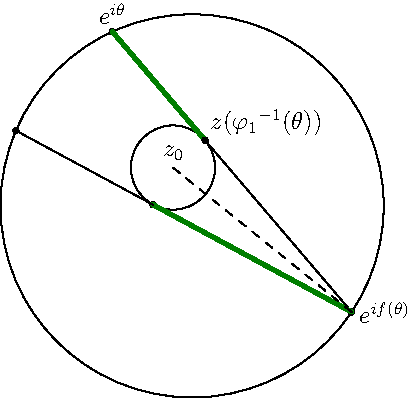
\includegraphics[width=5cm]{Cponcelet_1.pdf}
  % Cponcelet_1.pdf: 156x145 px, 72dpi, 5.50x5.12 cm, bb=0 0 156 145
\end{figure}
Considérons les longueurs des segments portés en gras.\newline
Notons $k(\theta) = \left|e^{i\theta} - z({\varphi_1}^{-1}(\theta)\right|$. L'autre segment est alors $k(f(\theta))$. Par symétrie par rapport à l'axe en pointillé:
\[
  k(f(\theta)) = \left|e^{if(\theta)} - z({\varphi_1}^{-1}(\theta)\right| \Rightarrow f' = \frac{h}{h\circ f} \text{ avec } h = \frac{1}{k}.
\]
La fonction $h$ vérifie les propriétés requises ($\Cont^{1}(\R, \R_{+}^{*})$ et $2\pi$-périodique) 
\item
\begin{enumerate}
  \item Par définition de la suite $(\theta_{n})_{n\in \N}$:
\[
  \forall n \in \N, \; \theta_n = f \circ f \circ \cdots \circ f (\theta) = f^n(\theta).
\]
De $\varphi \circ f \circ \varphi^{-1} = \tau_\alpha$, on tire
\begin{multline*}
  f = \varphi^{-1} \circ \tau_\alpha \circ \varphi \Rightarrow f^2 = (\varphi^{-1} \circ \tau_\alpha \circ \varphi) \circ (\varphi^{-1} \circ \tau_\alpha \circ \varphi)
  = \varphi^{-1} \circ {\tau_{\alpha}}^2 \circ \varphi \\
  \Rightarrow \cdots \Rightarrow f^n = \varphi^{-1} \circ {\tau_{\alpha}}^n \circ \varphi
  = \varphi^{-1} \circ {\tau_{n \alpha}} \circ \varphi \\
  \Rightarrow \theta_n = \varphi^{-1}(\varphi(\theta) + n\alpha)
  \Rightarrow \varphi(\theta_n) = \varphi(\theta) + n\alpha.
\end{multline*}

  \item D'après les questions précédentes, la suite $(z_{n})_{n\in \N}$ correspond à la suite définie dans l'introduction.
  \item Soit $p \in \N^*$. D'après les questions précédentes:
\begin{multline*}
  z_{n+p} = z_n \Leftrightarrow \theta_{n+p} \equiv \theta_n \mod 2\pi
  \Leftrightarrow \varphi(\theta_{n+p}) \equiv \varphi(\theta_n) \mod 2\pi\\
  \Leftrightarrow \varphi(\theta) + (n+p)\alpha \equiv \varphi(\theta) + n\alpha \mod 2\pi
  \Leftrightarrow p\alpha \equiv 0 \mod 2\pi.
\end{multline*}
On en déduit que la suite est périodique si et seulement si $\frac{\alpha}{\pi} \in \Q$. Ce nombre $\alpha$ ne dépend que de la fonction $f$ et pas du $\theta$ initial choisi. La périodicité est une propriété du cercle $\Gamma$ dans $\mathbb{D}$.
\end{enumerate}

\end{enumerate}
